% 261-837

La maggior parte della memoria secondaria nei computer moderni è costituita da \textbf{hard disk drive}, HDD, e dispositivi di \textbf{memoria non volatile}, NVM.

\paragraph{HDD} fanno ruotare piatti di materiale a rivestimento magnetico sotto testine di lettura-scrittura mobili:


\begin{itemize}
  \item I dischi ruotano da 60 a 250 volte al secondo
  \item La velocità di trasferimento è la velocità con cui i dati scorrono tra il disco e il computer, $\approx\,1$ Gb/sec
  \item Il tempo di posizionamento (tempo di accesso casuale) è il tempo necessario per spostare il braccio del disco al cilindro desiderato (seek time) e il tempo per far ruotare il settore desiderato sotto la testina (latenza rotazionale), da 3ms a 12ms
  \item Lo schianto della testina avviene quando la testina del disco entra in contatto con la superficie del disco -- molto grave
\end{itemize}

\begin{figure}[h!]
  \centering
  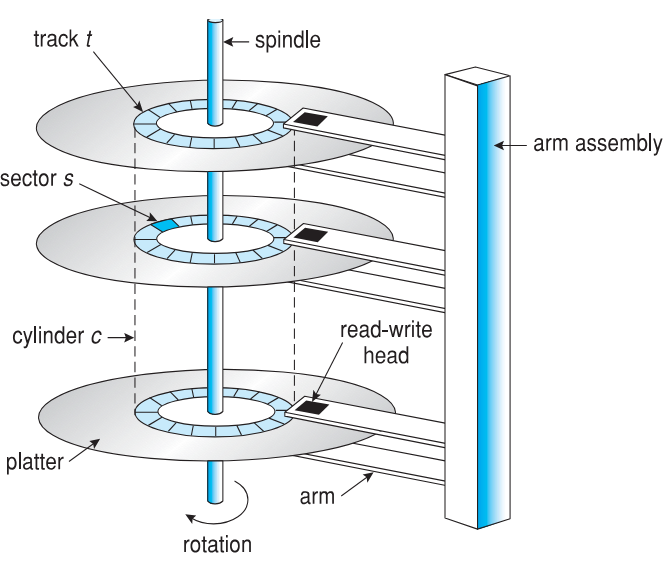
\includegraphics[width=0.75\linewidth]{content/OS_Internals/img/yys.png}
\end{figure}


\begin{equation*}
  \text{Latenza di accesso (tempo medio di accesso) = tempo medio di seek + latenza media}
\end{equation*}

Per un disco molto veloce: 3 ms + 2 ms = 5 ms.

\begin{equation*}
  \text{Tempo medio di I/O = tempo medio di accesso + (dati da trasferire / velocità di trasferimento) + overhead del controller}
\end{equation*}

\paragraph{Esempio: } trasferire un blocco da 4KB su un disco a 7200 RPM con un seek time medio di 5ms, velocità di trasferimento di 1Gb/sec e overhead del controller di 0.1ms.

\paragraph{}
A 7200 RPM = 120 giri/sec = 8.333ms/giro; nel caso peggiore bisogna attendere 1 rotazione completa, ma in media si attende mezza rotazione, pari a 4.17ms.


Tempo di trasferimento = 4KB / 1Gb/s * 8Gb / GB * 1GB / 10242KB = 32 / ($1024^2$) = 0.031 ms

Tempo medio di I/O per un blocco da 4KB = 5ms + 4.17ms + 0.1ms + 0.031ms = 9.301ms

\section{Dispositivi di Memoria Non Volatile}

L'NVM include solid-state drive e chiavette USB. Questi dispositivi sono più affidabili e \textbf{più veloci} degli HDD, ma più costosi.

La lettura e scrittura avviene in incrementi di pagina (come i settori), ma non si può sovrascrivere in-place: occorre prima cancellare, e le cancellazioni avvengono in incrementi di blocco più grandi. Questi dispositivi possono essere cancellati un numero limitato di volte, espresso come \textbf{drive writes per day}, DWPD.

\paragraph{}
L'SSD è un dispositivo complesso che integra un processore per verificare lo stato di tutti i settori, cancellare e scrivere blocchi, ecc.

\section{Algoritmi del Controller NAND Flash}



\begin{center}
  \begin{minipage}{0.65\linewidth}
    Poiche non e possibile sovrascrivere in-place, le pagine finiscono per contenere un mix di dati validi e non validi.
    Per tracciare quali blocchi logici sono validi, il controller mantiene una tabella \textbf{flash
      translation layer} (FTL).
    Implementa inoltre la \textbf{garbage collection} per liberare lo spazio occupato dalle pagine non valide.
    Riserva \textbf{overprovisioning} per fornire spazio di lavoro alla GC.
    Ogni cella ha una vita utile limitata, quindi e necessario il \textbf{wear leveling} per distribuire uniformemente le scritture.
  \end{minipage}%
  \hfill
  \begin{minipage}{0.3\linewidth}
    \centering
    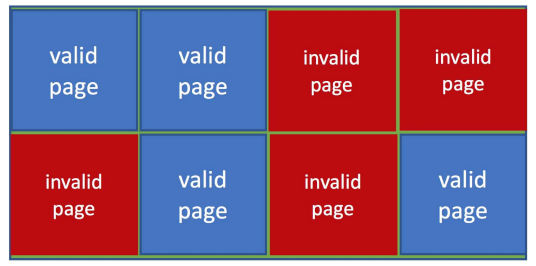
\includegraphics[width=\linewidth]{content/OS_Internals/images/2026-03-22-16-53-48.png}
  \end{minipage}
\end{center}


\section{Memoria Volatile}

La DRAM viene spesso usata come dispositivo di mass-storage; tecnicamente non e memoria secondaria
perche e volatile, ma puo ospitare file system ed essere usata come storage secondario molto veloce.

I RAM drive (chiamati anche RAM disk) si presentano come dispositivi a blocchi raw,
solitamente formattati con un file system.


I computer hanno gia buffering e caching via RAM: perche usare i RAM drive?

\begin{itemize}
  \item Cache e buffer sono allocati/gestiti da programmatore, sistema operativo e hardware
  \item I RAM drive sono sotto il controllo diretto dell'utente
  \item Sono presenti in tutti i principali sistemi operativi. Ad esempio Linux \texttt{/dev/ram}, MacOS \texttt{diskutil}
\end{itemize}

Sono usati come storage temporaneo ad alta velocita. I programmi possono condividere rapidamente grandi quantita di dati leggendo/scrivendo sul RAM drive.

\section{Struttura del Disco}


I dischi vengono indirizzati come grandi array monodimensionali di blocchi logici,
dove il blocco logico e la minima unita di trasferimento.
Il low-level formatting crea i blocchi logici sul supporto fisico.

L'array monodimensionale di blocchi logici viene mappato in modo sequenziale
nei settori del disco:

\begin{itemize}
  \item Il settore 0 e il primo settore della prima traccia del cilindro piu esterno
  \item La mappatura procede in ordine lungo quella traccia, poi sulle altre tracce dello stesso cilindro, quindi sui restanti cilindri dall'esterno verso l'interno
  \item L'indirizzamento logico-fisico dovrebbe essere semplice, salvo eccezioni dovute a bad sector e al numero non costante di settori per traccia
\end{itemize}

\subsection{Collegamento del Disco}

Lo storage host-attached viene raggiunto tramite porte di I/O collegate ai bus di I/O. Sono disponibili vari bus,
tra cui advanced technology attachment (ATA), serial ATA (SATA), eSATA, serial attached SCSI (SAS),
universal serial bus (USB) e fibre channel (FC). Il piu comune e SATA.

Poiche la NVM e molto piu veloce degli HDD, e stata introdotta una nuova interfaccia ad alte prestazioni,
NVM express (NVMe), che si collega direttamente al bus PCI.
I trasferimenti dati su bus sono gestiti da processori elettronici specializzati chiamati
controller (o host-bus adapter, HBA).

\begin{itemize}
  \item Un host controller lato computer del bus e un device controller lato dispositivo
  \item Il computer inserisce i comandi nell'host controller tramite porte di I/O memory-mapped; l'host controller invia messaggi al device controller e i dati sono trasferiti via DMA tra dispositivo e DRAM del computer
\end{itemize}


\section{Scheduling del Disco}

Il sistema operativo è responsabile dell'uso efficiente dell'hardware; per il disco ciò significa avere un accesso rapido e una buona \textbf{larghezza di banda} del disco. La \textbf{bandwidth} è il numero totale di byte trasferiti, diviso per il tempo totale tra la prima richiesta di servizio e il completamento dell'ultimo trasferimento.

\paragraph{}

Le sorgenti delle richieste di I/O su disco sono molte: OS, processi di sistema, processi utente; includono tutte scrittura/lettura, indirizzo del disco, indirizzo di memoria, numero di settori da trasferire. L'OS mantiene una coda di richieste per dispositivo.

In passato l'HD non era sofisticato come oggi; l'OS doveva occuparsi di tutto: gestione della coda e scheduling della testina del disco. Ora il controllo è affidato all'HD e l'OS deve solo passare gli indirizzi dei blocchi, lasciando che il disco ordini le richieste.

\paragraph{Esempio: } vogliamo gestire la seguente lista di richieste usando diversi algoritmi di scheduling:

\begin{itemize}
  \centering
  \item[] 98, 183, 37, 122, 14, 124, 65, 67
\end{itemize}

La testina parte dalla posizione 53

\newpage
\subsection{FCFS}

\begin{figure}[h!]
  \centering
  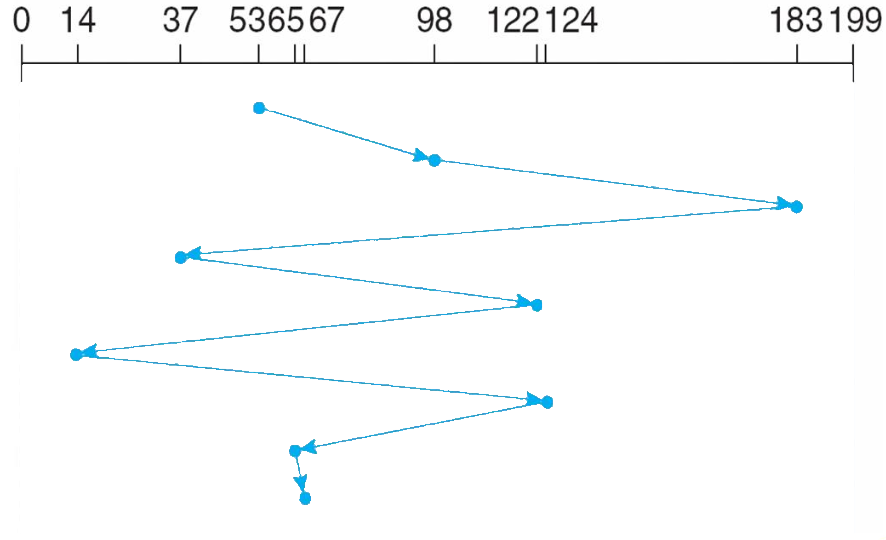
\includegraphics[width=0.5\linewidth]{content/OS_Internals/img/Immagine 2024-05-22 183104.png}
\end{figure}

\subsection{SCAN - algoritmo dell'ascensore}

Il braccio del disco parte da un'estremità e si sposta verso l'altra. Questo non è equo: gli ultimi valori devono aspettare molto a lungo.

\begin{figure}[h!]
  \centering
  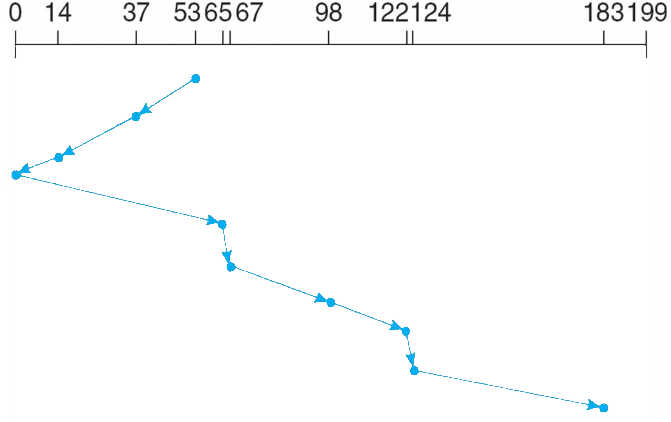
\includegraphics[width=0.5\linewidth]{content/OS_Internals/img/Immagine 2024-05-22 183628.png}
\end{figure}

\begin{tcolorbox}
  \textbf{Nota:} non ci sono richieste da 0 a 65, quindi possiamo saltare quella zona.
\end{tcolorbox}

L'algoritmo SCAN e talvolta chiamato algoritmo dell'ascensore.
Nell'illustrazione il movimento totale della testina e di 208 cilindri.
Si noti pero che, se le richieste sono distribuite uniformemente, la densita maggiore si trova all'estremita opposta del disco,
e quelle richieste attendono piu a lungo.



\subsection{C-SCAN}
Fornisce un tempo di attesa più uniforme rispetto a SCAN: la testina si sposta da un'estremità del disco all'altra, servendo le richieste man mano che procede. Quando raggiunge l'altra estremità, tuttavia, ritorna immediatamente all'inizio del disco senza servire alcuna richiesta durante il percorso di ritorno.


\begin{figure}[h!]
  \centering
  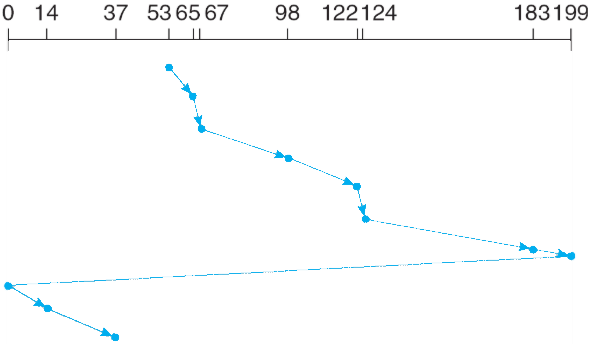
\includegraphics[width=0.5\linewidth]{content/OS_Internals/img/Immagine 2024-05-22 184919.png}
\end{figure}

\newpage
\subsection{Scelta dell'Algoritmo di Scheduling del Disco}

\begin{itemize}
  \item FCFS è comune e ha un'attrattiva naturale
  \item SCAN e C-SCAN hanno prestazioni migliori per sistemi con un carico elevato sul disco
\end{itemize}

Linux implementa lo scheduler deadline

\begin{itemize}
  \item[-] Mantiene code separate per lettura e scrittura
  \item[-] Per impostazione predefinita, i batch di lettura hanno la precedenza sui batch di scrittura, poiché le applicazioni tendono a bloccarsi sulle operazioni di I/O in lettura
  \item[-] Schedula i batch di lettura e scrittura per l'esecuzione in ordine crescente di indirizzamento logico dei blocchi (LBA)
  \item[-] Dopo ogni batch, seleziona naturalmente i batch di lettura se presenti, ma controlla anche da quanto tempo le operazioni di scrittura sono in attesa (per evitare la starvation)
  \item[-] Schedula il successivo batch di lettura o scrittura secondo necessità
  \item[-] Tipicamente, se un batch di lettura è in attesa da più di 500ms, ottiene la priorità sulla scrittura
\end{itemize}

Questo scheduler è adatto alla maggior parte dei casi d'uso, in particolare quelli in cui le
operazioni di scrittura sono prevalentemente \textbf{asincrone}.


\section{Pianificazione per la NVM}
Non vi sono testine del disco né latenza rotazionale, ma c'è ancora margine per l'ottimizzazione. L'NVM è migliore nell'I/O casuale, l'HDD nell'I/O sequenziale; le operazioni di input/output al secondo (IOPS) sono molto più elevate con NVM (centinaia di migliaia vs centinaia).


\section{Rilevamento e Correzione degli Errori}

Un aspetto fondamentale di molte parti dell'informatica è il \textbf{Rilevamento e Correzione degli Errori}.

Il \textbf{rilevamento degli errori} determina se si è verificato un problema; viene spesso implementato tramite bit di parità.

La parità è una forma di checksum; un altro metodo di rilevamento errori è il controllo di ridondanza ciclica (CRC), che usa una funzione hash per rilevare errori su più bit.

\paragraph{}

Il \textbf{codice di correzione degli errori}, ECC, non solo rileva, ma può anche correggere alcuni errori; gli errori soft sono correggibili, quelli hard vengono rilevati ma non corretti.


\subsection{Gestione dei dispositivi di storage}

\textbf{Il low-level formatting}, o \textbf{formattazione fisica}, divide un disco in settori che il controller può leggere e scrivere. Ogni settore contiene un'intestazione, i dati e il codice di correzione degli errori. In genere ospita 512 byte di dati, ma il valore può essere configurabile.

Per usare un disco per i file, il sistema operativo deve comunque registrare sul disco le proprie strutture dati:

\begin{itemize}
  \item \textbf{Partizionare} il disco in uno o più gruppi di cilindri, ognuno trattato come disco logico
  \item Eseguire la \textbf{formattazione logica}, o “creare un file system”
\end{itemize}

Per aumentare l'efficienza molti file system raggruppano i blocchi in cluster. L'I/O sul disco avviene in blocchi, quello sui file nei cluster.


\paragraph{}

La \textbf{partizione di boot/root} contiene il sistema operativo; le altre partizioni possono contenere altri sistemi operativi, altri file system, o essere raw. La partizione può essere \textbf{montata} al boot, automaticamente o manualmente.

Al momento del montaggio, viene verificata la consistenza del file system e la correttezza di tutti i metadati.

\begin{itemize}
  \item[] Se non corretta, correggere e riprovare
  \item[] Se corretta, aggiungere alla tabella di montaggio e consentire l'accesso
\end{itemize}

Il boot block, o un programma di gestione del boot per sistemi multi-OS, può puntare al volume di boot o al boot loader, ovvero un insieme di blocchi che contengono il codice necessario per caricare il kernel dal file system.

Il boot block inizializza il sistema ed è memorizzato in ROM, firmware. Il programma Bootstrap loader è memorizzato nei boot block della partizione di boot: il master boot record MBR.

\begin{figure}[h!]
  \centering
  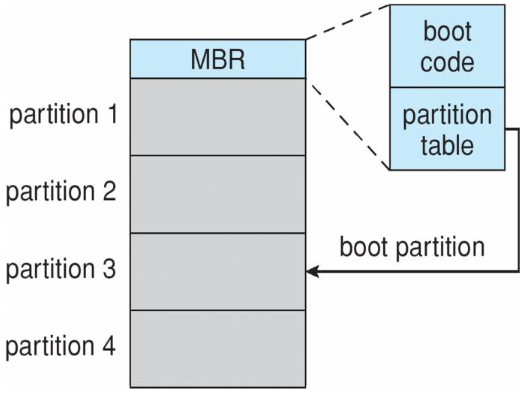
\includegraphics[width=0.37\linewidth]{content/OS_Internals/img/fhmgmfgzh.png}
  \caption{Avvio dallo storage secondario in Windows}
\end{figure}

\subsection{Gestione dello Spazio di Swap}
Utilizzato per spostare interi processi o pagine dalla DRAM all'archiviazione secondaria quando la DRAM non è sufficiente per tutti i processi. Il sistema operativo fornisce la \textbf{gestione dello spazio di swap}:

\begin{itemize}
  \item L'archiviazione secondaria è più lenta della DRAM, quindi è importante ottimizzare le prestazioni
  \item Di solito sono possibili più spazi di swap, riducendo il carico di I/O su ogni singolo dispositivo
  \item È preferibile avere dispositivi dedicati
  \item Può essere in una partizione raw o in un file all'interno di un file system (per comodità)
\end{itemize}


\begin{figure}[h!]
  \centering
  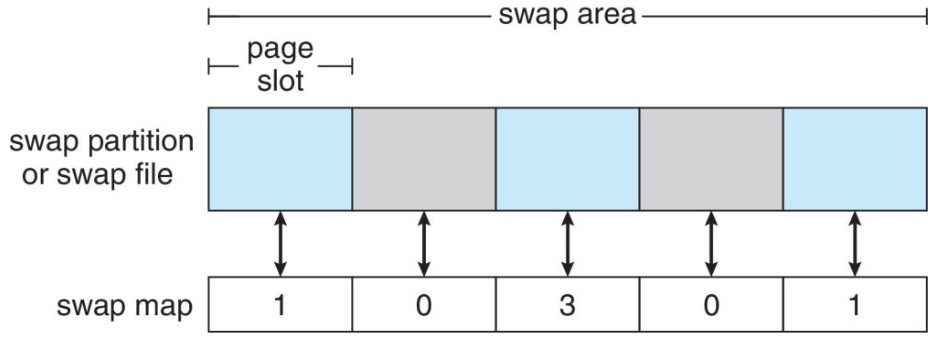
\includegraphics[width=0.55\linewidth]{content/OS_Internals/img/amrjkyt.png}
  \caption{Strutture dati per lo swapping nei sistemi Linux}
\end{figure}


\newpage
\subsection{Collegamento dello Storage all'Host}

I computer accedono allo storage in tre modi:

\begin{itemize}
  \item[--] collegato all'host
  \item[--] collegato in rete
  \item[--] cloud
\end{itemize}

L'accesso collegato all'host avviene tramite porte I/O locali, usando una delle varie tecnologie per collegare molti dispositivi (USB, LAN...).

\subsubsection{Storage Collegato in Rete: NAS}

Il network-attached storage (NAS) è uno storage reso disponibile tramite rete anziché tramite un canale locale (come un bus). \textbf{NFS} e \textbf{CIFS} sono protocolli comuni, implementati tramite Remote Procedure Call (RPC) tra host e storage, tipicamente su TCP o UDP su rete IP.

\begin{figure}[h!]
  \centering
  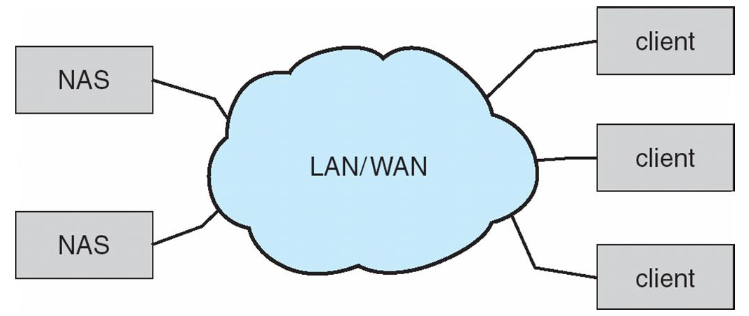
\includegraphics[width=0.5\linewidth]{content/OS_Internals/img/tdmng.png}
  \caption{NAS}
\end{figure}

\subsection{Archiviazione Cloud}

Simile al NAS, fornisce accesso allo storage tramite rete. A differenza del NAS, viene acceduto tramite Internet o WAN verso data center remoti.

Il NAS viene presentato come un normale file system, mentre lo storage cloud è basato su API, con programmi che usano le API per fornire l'accesso. Si usano le API a causa della latenza e degli scenari di guasto (i protocolli NAS non funzionerebbero bene).


\subsection{Storage Array}

Si possono collegare semplicemente dischi singoli oppure array di dischi. Questo evita lo svantaggio del NAS legato al consumo di banda di rete.
Uno storage array ha uno o piu controller e offre funzionalita ai sistemi host collegati.

\begin{itemize}
  \item Porte per connettere gli host all'array
  \item Memoria e software di controllo (talvolta anche NVRAM, ecc.)
  \item Da pochi dischi fino a migliaia
  \item RAID, hot spare, hot swap (discussi in seguito)
  \item Storage condiviso $\rightarrow$ maggiore efficienza
  \item Funzionalita tipiche di alcuni file system: snapshots, cloni, thin provisioning, replication,
        deduplication, ecc.
\end{itemize}


\subsection{Storage Area Network  - SAN}


\begin{center}
  \begin{minipage}{0.65\linewidth}
    Comune negli ambienti di storage di grandi dimensioni: piu host collegati a piu
    storage array, con elevata flessibilita.
  \end{minipage}%
  \hfill
  \begin{minipage}{0.3\linewidth}
    \centering
    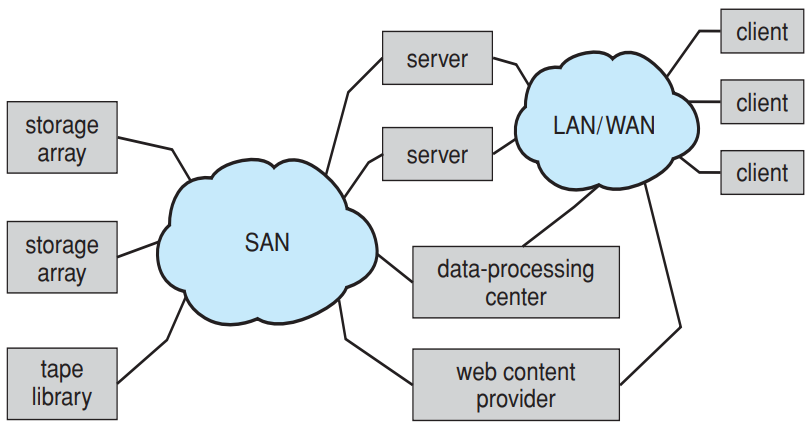
\includegraphics[width=\linewidth]{content/OS_Internals/images/2026-03-22-17-19-31.png}
  \end{minipage}
\end{center}

Una SAN e composta da uno o piu storage array collegati a uno o piu switch Fibre
Channel oppure a una rete InfiniBand (IB).
Anche gli host si collegano a questi switch.

Lo storage viene reso disponibile tramite LUN,
con masking da specifici array verso specifici server.
E facile aggiungere o rimuovere storage, aggiungere nuovi host e assegnare loro capacita.
Perche mantenere reti separate per storage e comunicazioni?
Si considerino iSCSI e FCoE.


\subsection{Array Ridondante di Dischi Indipendenti - RAID}

RAID - più dischi forniscono affidabilità tramite ridondanza.

\begin{itemize}
  \item Aumenta il \textbf{tempo medio al guasto}.
  \item \textbf{Tempo medio di riparazione} - periodo di esposizione durante il quale un altro guasto potrebbe causare perdita di dati
  \item \textbf{Tempo medio alla perdita di dati} basato sui fattori precedenti
\end{itemize}


Se i dischi speculari si guastano indipendentemente, si consideri un disco con 100.000 ore di tempo medio al guasto e 10 ore di tempo medio di riparazione. Il tempo medio alla perdita di dati è:

\begin{equation*}
  \text{MTDL } = 100\,000^2 / (2*10) = 500 * 10^6 \text{ hours or 57 000 years! }
\end{equation*}

RAID mirror: 2 dischi

Con 2 dischi in mirror: $\mathrm{MTTF}_1 = \mathrm{MTTF}/2$ e $P_2 = \mathrm{MTTR}/\mathrm{MTTF}$.

\begin{equation*}
  \mathrm{MTTDL} = \frac{\mathrm{MTTF}^2}{2\cdot\mathrm{MTTR}} = \frac{(100000)^2}{2\cdot10} = 5\cdot10^8\ \text{hours} \approx 57000\ \text{years}
\end{equation*}

\vspace{1cm}

Diversi miglioramenti nelle tecniche di utilizzo dei dischi coinvolgono l'uso di
più dischi che lavorano in modo cooperativo.

\newpage

Il \textbf{striping} del disco utilizza un gruppo di dischi come un'unica unità di archiviazione. Il RAID è organizzato in sei diversi livelli.

I sistemi RAID migliorano le prestazioni e l'affidabilità dello storage memorizzando dati ridondanti.


\begin{itemize}
  \item Il \textbf{mirroring} o shadowing (\textbf{RAID 1}) mantiene una copia duplicata di ogni disco
  \item Mirror striped (\textbf{RAID 1+0}) o stripe mirror (\textbf{RAID 0+1}) offre alte prestazioni e alta affidabilità
  \item La parità a blocchi interlacciati (\textbf{RAID 4, 5, 6}) usa molta meno ridondanza
\end{itemize}

Il RAID all'interno di un array di storage può comunque fallire se l'array si guasta, quindi la replica automatica dei dati tra array è comune. Spesso un piccolo numero di dischi hot-spare viene lasciato non allocato, pronto a sostituire automaticamente un disco guasto e a ricostruire i dati su di esso.


\begin{figure}[h!]
  \begin{minipage}{0.75\linewidth}
    \begin{minipage}[h!]{0.47\textwidth}
      \centering
      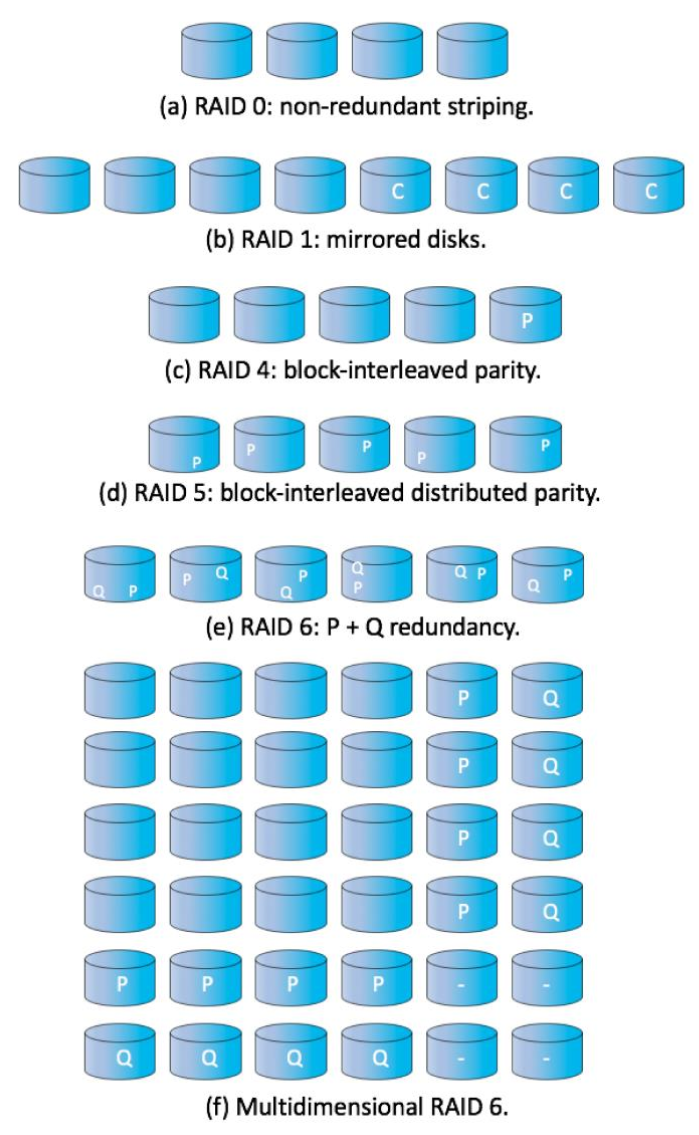
\includegraphics[width=1\linewidth]{content/OS_Internals/img/zmfdg.png}
      \caption{Schemi RAID}
    \end{minipage}
    \begin{minipage}[h!]{0.47\textwidth}
      \centering
      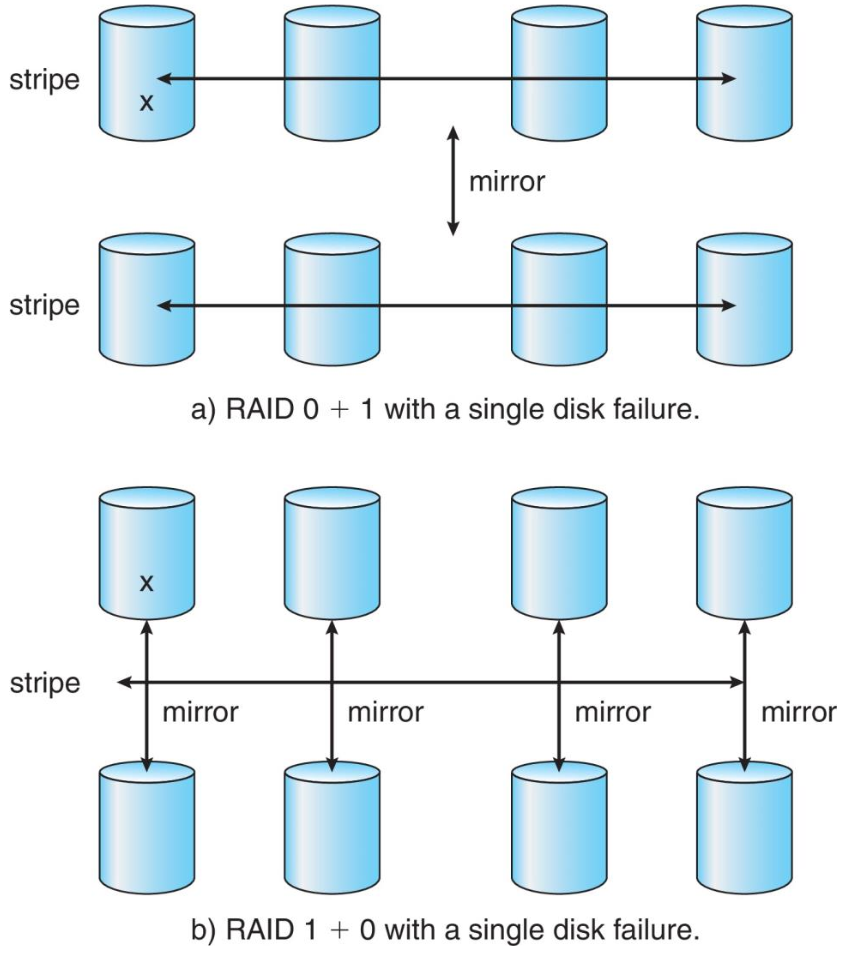
\includegraphics[width=1\linewidth]{content/OS_Internals/img/zmnfdg.png}
    \end{minipage}
  \end{minipage}
\end{figure}


\section{Altre Funzionalita}
Indipendentemente da dove sia implementato il RAID, si possono aggiungere altre funzionalita utili.
Uno snapshot e una vista del file system prima che avvenga un insieme di modifiche
(cioe in uno specifico istante temporale).

La replication e la duplicazione automatica delle scritture tra siti separati,
utile per ridondanza e disaster recovery. Puo essere sincrona o asincrona.

Un disco hot spare e un disco non usato normalmente, che entra in funzione automaticamente
se un disco si guasta, per sostituirlo e ricostruire il set RAID quando possibile.
Questo riduce il tempo medio di riparazione.


\section{Estensioni}



\begin{center}
  \begin{minipage}{0.65\linewidth}
    Il solo RAID non previene ne rileva la
    corruzione dei dati o altri errori: copre soprattutto i
    guasti dei dischi. Solaris ZFS aggiunge checksum su tutti i dati
    e i metadati.
    I checksum sono mantenuti insieme ai puntatori agli oggetti,
    per verificare che l'oggetto sia quello corretto
    e che non sia stato modificato.

    ZFS puo rilevare e correggere la corruzione
    di dati e metadati. Inoltre elimina il concetto tradizionale di volumi e partizioni.

    I dischi sono allocati in \textbf{pool}. I file system che usano un pool lo condividono,
    allocando e rilasciando spazio in modo simile alle chiamate
    \verb|malloc()| e \verb|free()| per la memoria.
  \end{minipage}%
  \hfill
  \begin{minipage}{0.3\linewidth}
    \centering
    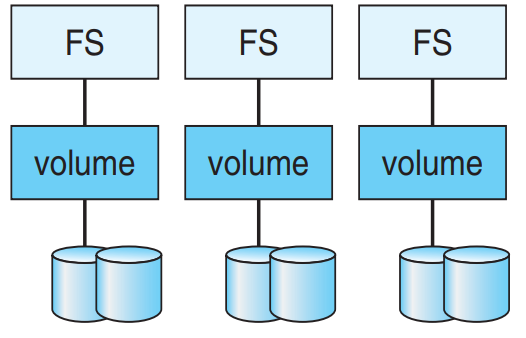
\includegraphics[width=\linewidth]{content/OS_Internals/images/2026-03-22-17-32-18.png}
    \captionof{figure}{Volumi e file system tradizionali}
  \end{minipage}
\end{center}

\begin{center}
  \begin{minipage}{0.65\linewidth}

  \end{minipage}%
  \hfill
  \begin{minipage}{0.3\linewidth}
    \centering
    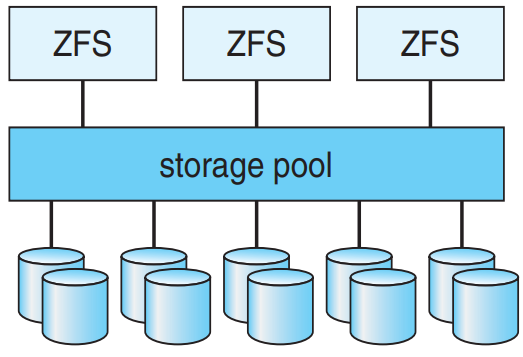
\includegraphics[width=\linewidth]{content/OS_Internals/images/2026-03-22-17-32-56.png}
    \captionof{figure}{ZFS e storage a pool}
  \end{minipage}
\end{center}


\section{Object Storage}
Nel calcolo general-purpose, i file system tradizionali non sono sempre sufficienti su scala molto grande.
Un approccio alternativo e partire da uno storage pool e inserirvi oggetti.

Un oggetto e semplicemente un contenitore di dati. Non esiste navigazione del pool per trovare oggetti
(niente strutture a directory, pochi servizi): e un modello orientato alle macchine, non all'utente.

Sequenza tipica:

\begin{itemize}
  \item Creare un oggetto nel pool e ricevere un object ID
  \item Accedere all'oggetto tramite quell'ID
  \item Eliminare l'oggetto tramite quell'ID
\end{itemize}

Software di gestione dell'object storage come Hadoop file system
(HDFS) e Ceph determinano dove memorizzare gli oggetti e come proteggerli,
tipicamente mantenendo N copie su N sistemi nel cluster di object storage.
Il modello e scalabile orizzontalmente, content-addressable e non strutturato.



\chapter{Interfaccia del File System}

\section{Cos'è un File?}

Spazio di indirizzamento logico contiguo. Tipi:

\begin{itemize}
  \item File di Dati
        \begin{itemize}
          \item Numerico
          \item Carattere
          \item Binario
        \end{itemize}
  \item File di Programma
\end{itemize}

\begin{figure}[h!]
  \centering
  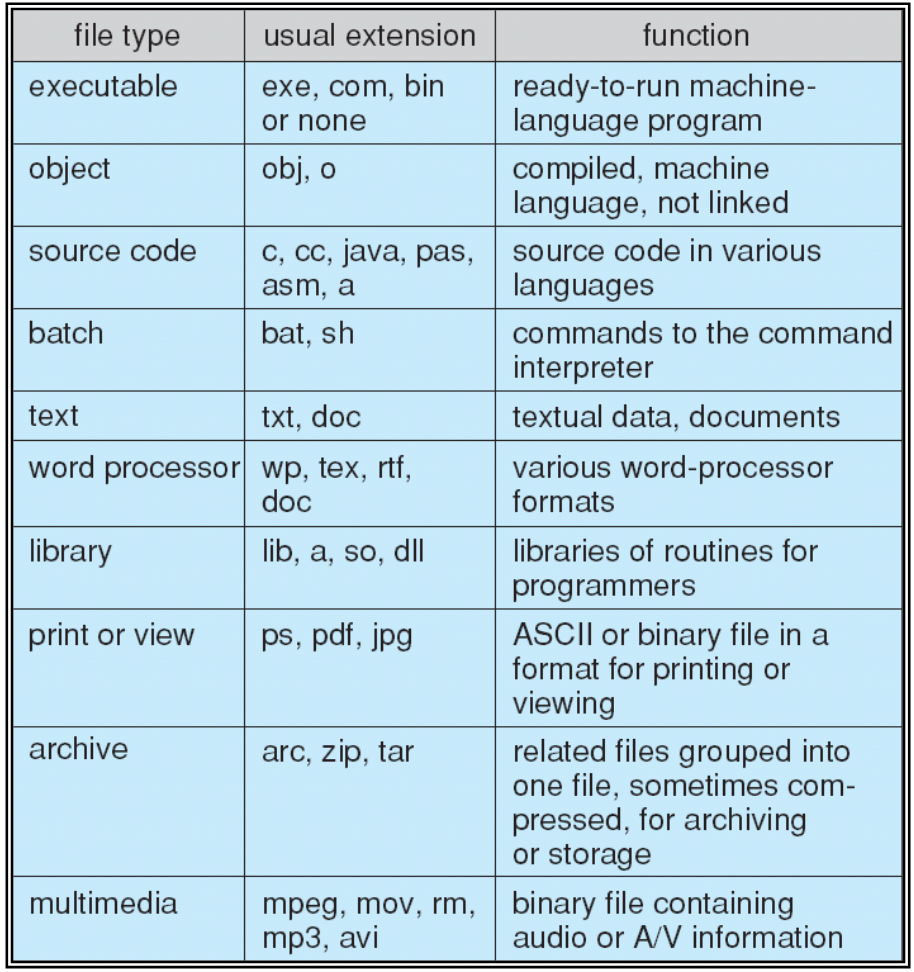
\includegraphics[width=0.5\linewidth]{content/OS_Internals/img/fgnfnfg.png}
  \caption{Tipi di file}
\end{figure}


\newpage
\subsection{Attributi del File}

\begin{itemize}
  \item \textbf{Nome} - è la sola informazione mantenuta in forma leggibile dall'uomo
  \item \textbf{Identificatore} - tag unico (numero) che identifica il file all'interno del file system
  \item \textbf{Tipo} - necessario per i sistemi che supportano tipi diversi
  \item \textbf{Posizione} - puntatore alla posizione del file sul dispositivo
  \item \textbf{Dimensione} - dimensione corrente del file
  \item \textbf{Protezione} - controlla chi può leggere, scrivere, eseguire
  \item \textbf{Ora}, \textbf{data} e \textbf{identificazione utente} - dati per protezione, sicurezza e monitoraggio dell'uso
\end{itemize}

Le informazioni sui file sono conservate nella \textbf{struttura delle directory}, mantenuta sul disco. Molte varianti, tra cui attributi estesi del file come il checksum.

\subsection{Struttura del File}

\begin{itemize}
  \item Nessuna - sequenza di parole, byte
  \item Struttura semplice - Righe, lunghezza fissa, lunghezza variabile...
  \item Strutture complesse - Documento formattato, File di caricamento rilocabile
\end{itemize}

Le ultime due strutture possono essere simulate con la prima inserendo opportuni caratteri di controllo.

La decisione sulla struttura spetta all'\textbf{OS} o al \textbf{Programma}.

\section{Accesso e Operazioni sui File}

Sono necessari diversi dati per gestire i \textbf{file aperti}:

\begin{itemize}
  \item \textbf{Tabella dei file aperti}: traccia i file aperti
  \item Puntatore al file: puntatore all'ultima posizione di lettura/scrittura, specifico per ogni processo che ha il file aperto
  \item \textbf{Contatore di aperture del file}: contatore del numero di volte in cui un file è aperto, per consentire la rimozione dei dati dalla tabella dei file aperti quando l'ultimo processo lo chiude
  \item Posizione del file su disco: cache delle informazioni di accesso ai dati
  \item Diritti di accesso: informazioni sulla modalità di accesso per processo
\end{itemize}

\subsection{Blocco dei File}
Fornito da alcuni \textbf{sistemi operativi} e file system. Simile ai lock lettore-scrittore.

\textbf{Lock condiviso} simile al lock lettore - più processi possono acquisirlo contemporaneamente
\textbf{Lock esclusivo} simile al lock scrittore

\paragraph{}

\textbf{Obbligatorio} - l'accesso è negato in base ai lock detenuti e richiesti
\textbf{Consultivo} - i processi possono conoscere lo stato dei lock e decidere come procedere

\paragraph{Esempio: } provare a scrivere un file già aperto in Excel genera un errore; aprire un file in gedit di solito non lo fa.

\subsection{Metodi di Accesso}

Un file è un \textbf{record logico} di lunghezza fissa:

\begin{itemize}
  \item Accesso Sequenziale
  \item Accesso Diretto
  \item Altri Metodi di Accesso
\end{itemize}

\subsubsection{Accesso Sequenziale}
Operazioni: \texttt{read next}, \texttt{write next}, reset; nessuna lettura dopo l'ultima scrittura (rewrite) e nessuna operazione di seek.


\begin{figure}[h!]
  \centering
  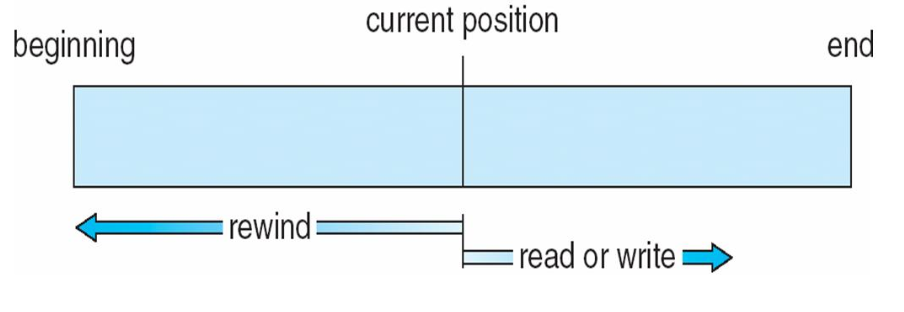
\includegraphics[width=0.45\linewidth]{content/OS_Internals/img/andfg.png}
  \caption{Accesso sequenziale}
\end{figure}

\subsubsection{Accesso Diretto}
Operazioni: leggi n, scrivi n, Reset, Posiziona (seek) a n. n = numero di blocco relativo

\begin{figure}[h!]
  \centering
  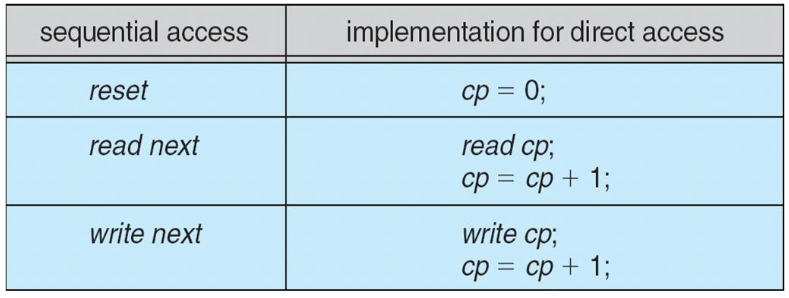
\includegraphics[width=0.5\linewidth]{content/OS_Internals/img/dbfs.png}
  \caption{Accesso diretto}
\end{figure}

\subsubsection{Accesso Sequenziale vs Diretto}


\begin{figure}[h!]
  \centering
  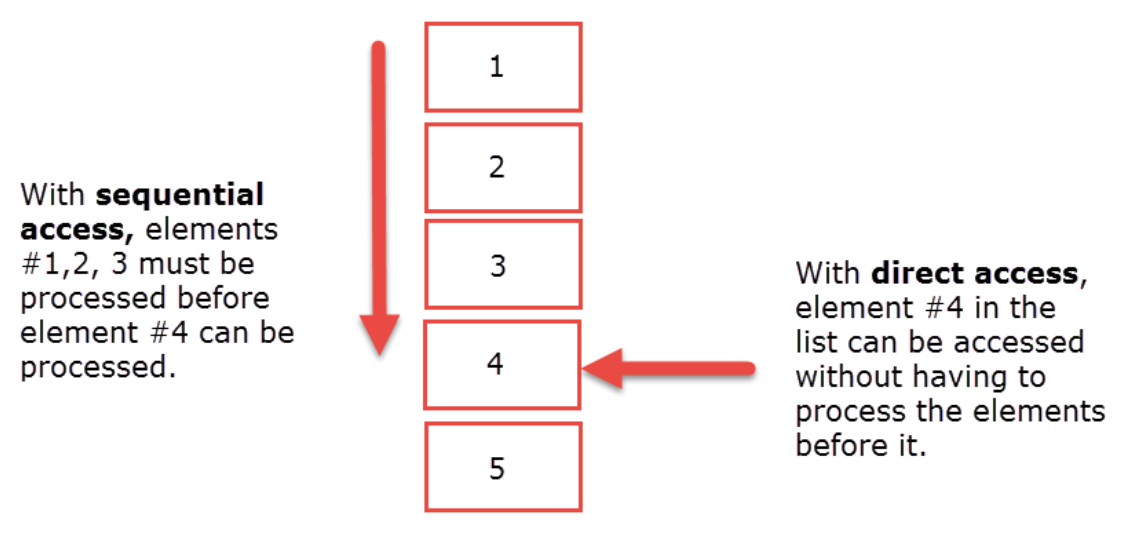
\includegraphics[width=0.5\linewidth]{content/OS_Internals/img/mhfg.png}
\end{figure}

\subsubsection{Altri Metodi di Accesso}

Possono esistere altri metodi di accesso costruiti sopra i metodi di base. Generalmente comportano la creazione di un indice per il file. L'indice viene mantenuto in memoria per la rapida individuazione della posizione dei dati
(si pensi al codice Universal Product Code (UPC) con i relativi record di dati).

Se l'indice è troppo grande, si crea un indice in memoria, che è un indice di un indice su disco.
\paragraph{}
Il metodo sequenziale ad accesso indicizzato di IBM (ISAM)

\begin{itemize}
  \item Piccolo indice master, punta ai blocchi su disco dell'indice secondario
  \item Il file è mantenuto ordinato su una chiave predefinita
  \item Tutto gestito dall'OS
  \item Un motore simile, MyISAM, è un modo per indicizzare i DB MySQL
\end{itemize}

\begin{figure}[h!]
  \centering
  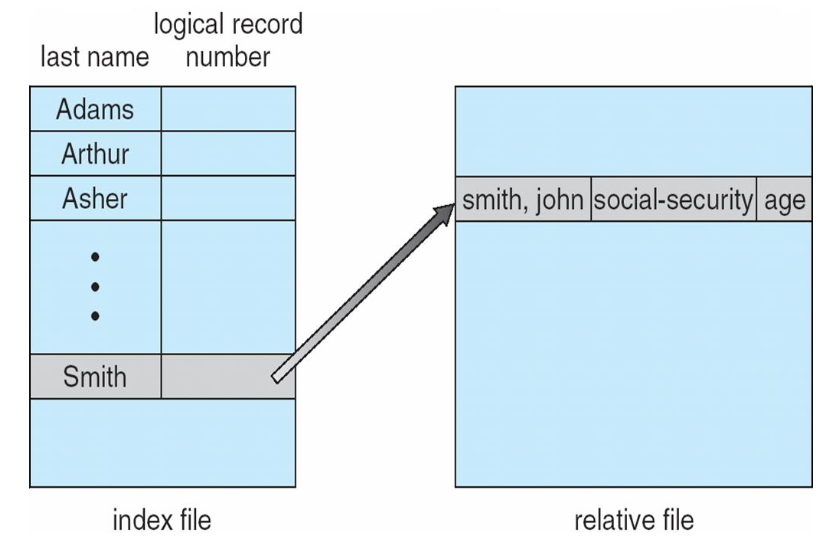
\includegraphics[width=0.5\linewidth]{content/OS_Internals/img/dfb.png}
\end{figure}

\section{File Mappati in Memoria}

Invece di accedere ai file di dati dall'HD ad ogni accesso, i file di dati possono essere paginati in memoria come i file di processo, risultando in accessi molto più veloci.

Si può vederlo come il "paging" di un file = una tabella delle pagine per file, eccetto ovviamente quando si verificano page-fault. Questo è noto come memory-mapping di un file.

\paragraph{}
Un file viene mappato su un intervallo di indirizzi all'interno dello spazio di indirizzamento virtuale di un processo e poi paginato secondo necessità usando il normale sistema di demand paging. Può essere usato per caricare un file da 10 GB con soli 2 GB di RAM disponibili!

Le scritture sul file vengono effettuate sui frame di pagina in memoria e non vengono immediatamente scritte su disco. Ecco perché è importante eseguire la \texttt{close()} su un file al termine della scrittura.

In questo modo i dati possono essere scritti su disco in sicurezza e i frame di memoria possono essere liberati per altri scopi.


\begin{figure}[h!]
  \centering
  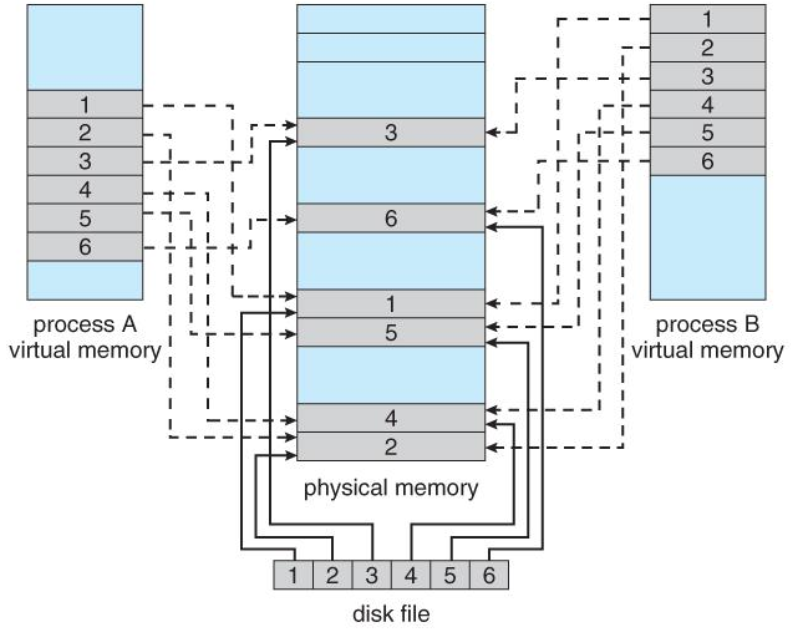
\includegraphics[width=0.5\linewidth]{content/OS_Internals/img/mfh.png}
  \caption{File mappati in memoria}
\end{figure}

\newpage
\section{Dischi e File System}

Dalla lezione precedente:
\begin{itemize}
  \item I dischi possono essere suddivisi in partizioni
  \item I dischi o le partizioni possono essere protetti da RAID contro i guasti
  \item Le partizioni sono note anche come minidisk, slice
\end{itemize}

Un file system governa l'organizzazione e l'accesso ai file.

L'entità contenente il file system è nota come volume; un disco o una partizione formattata è un volume.

Il disco o la partizione può essere usato grezzo (raw) - senza file system - oppure formattato con un file system. Ogni volume contenente un file system traccia anche le informazioni di quel file system nella directory del dispositivo o nella tabella dei contenuti del volume. Oltre ai file system di uso generale, esistono molti file system speciali, spesso tutti all'interno dello stesso sistema operativo o computer.

\subsection{Tipi di File System}
Parliamo principalmente di file system di uso generale, ma i sistemi spesso hanno molti file system, sia di uso generale sia speciali.

Si consideri Solaris, che ha:

\begin{itemize}
  \item tmpfs - FS volatile basato su memoria per I/O rapido e temporaneo
  \item objfs - interfaccia nella memoria del kernel per ottenere i simboli del kernel per il debugging
  \item ctfs - file system dei contratti per la gestione dei daemon
  \item lofs - file system loopback che consente l'accesso a un FS al posto di un altro
  \item procfs - interfaccia del kernel alle strutture dei processi
  \item ufs, zfs - file system di uso generale
\end{itemize}

Anche Linux ha più file system.


\section{Struttura delle Directory}
Una raccolta di nodi contenenti informazioni su tutti i file


\begin{figure}[h!]
  \centering
  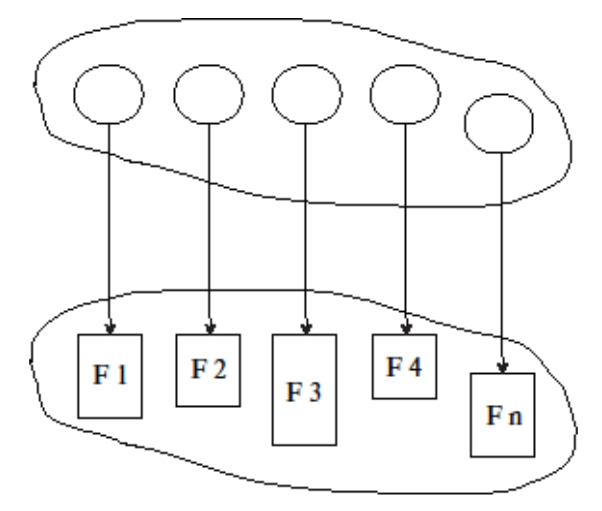
\includegraphics[width=0.4\linewidth]{content/OS_Internals/img/jhg.png}
\end{figure}

Sia la struttura delle directory che i file risiedono sul disco. Le informazioni delle directory si trovano di solito in cima a una partizione.

\begin{figure}[h!]
  \centering
  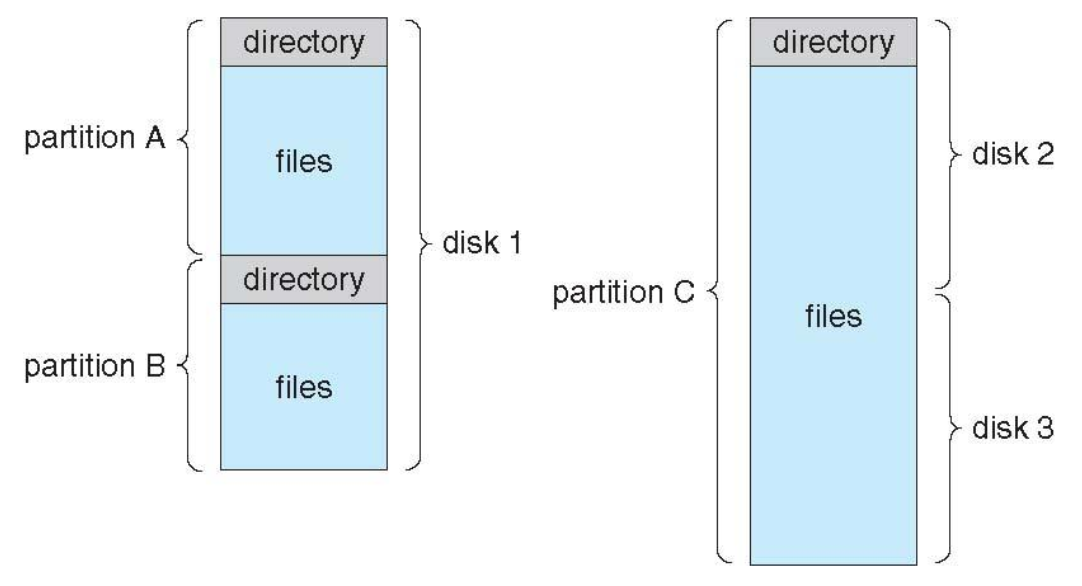
\includegraphics[width=0.5\linewidth]{content/OS_Internals/img/dbgnf.png}
\end{figure}

Le operazioni eseguite sulla Directory sono molte: ricerca di un file, creazione di un file, eliminazione di un file, elenco dei contenuti di una directory, rinomina di un file, navigazione del file system verso sottodirectory o directory padre.

\subsection{Organizzazione delle Directory}

La directory è organizzata logicamente per prestazioni, usabilità e controllo degli accessi.
In particolare:

\begin{itemize}
  \item Efficienza - individuare rapidamente un file
  \item Denominazione - comoda per gli utenti: due utenti possono avere lo stesso nome per file diversi; lo stesso file può avere più nomi diversi
  \item Raggruppamento - raggruppamento logico dei file per proprietà (es. tutti i programmi Java, tutti i giochi...)
\end{itemize}

\subsection{Directory a Singolo Livello}

\begin{figure}[h!]
  \centering
  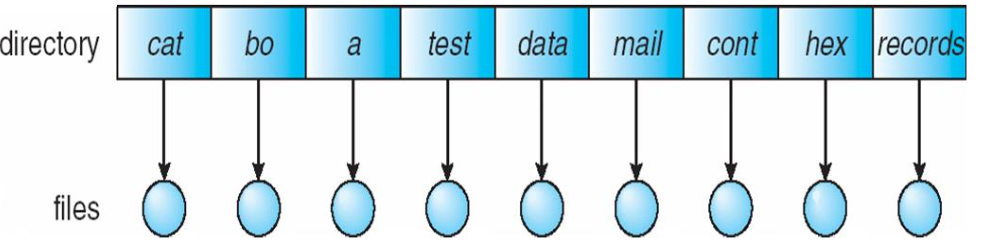
\includegraphics[width=0.5\linewidth]{content/OS_Internals/img/dfgnb.png}
  \caption{Una singola directory per tutti gli utenti}
\end{figure}

Molti problemi: il problema della denominazione e il problema del raggruppamento ne sono esempi.

\subsection{Directory a Due Livelli}

\begin{figure}[h!]
  \centering
  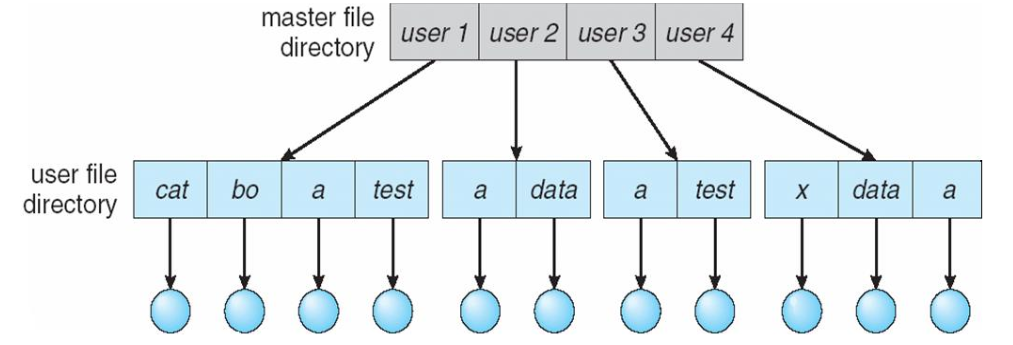
\includegraphics[width=0.5\linewidth]{content/OS_Internals/img/fng.png}
  \caption{Directory separata per ogni utente}
\end{figure}

Caratteristiche: Percorso lungo (negativo), Possibilità di avere lo stesso nome di file per utenti diversi (neutro), Ricerca efficiente (positivo), Nessuna capacità di raggruppamento (negativo)

\newpage
\subsection{Directory ad Albero}


\begin{figure}[h!]
  \begin{minipage}[h!]{0.47\textwidth}
    \centering
    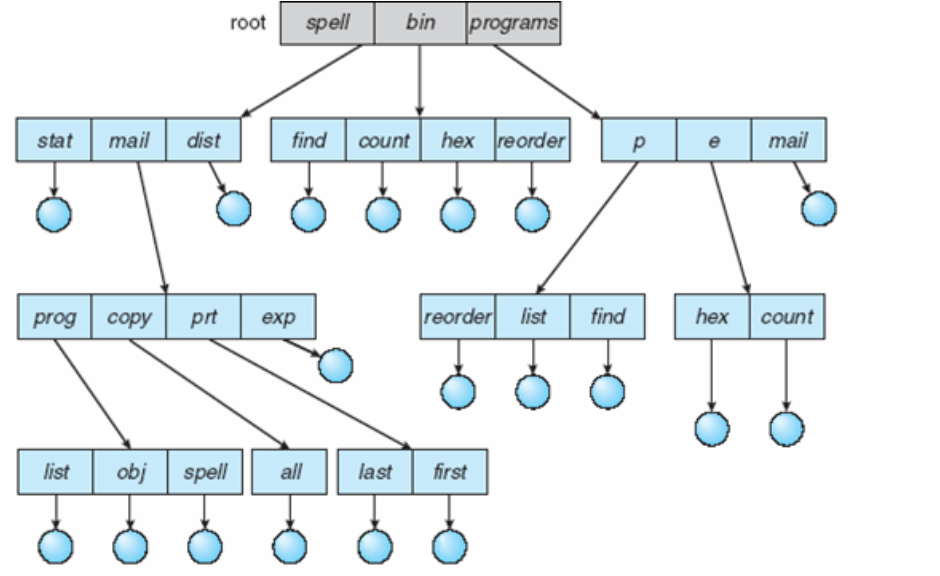
\includegraphics[width=1\linewidth]{content/OS_Internals/img/dfsbv.png}
  \end{minipage}
  \begin{minipage}[h!]{0.47\textwidth}
    \centering
    \begin{tabular}{c|c}
      Pro               & Contro                                \\
      \hline
      Generale          & Inefficiente                          \\
      Scalabile         & Nessuna condivisione di file          \\
      Facile da cercare & Duplicazione di file in più directory \\
    \end{tabular}

  \end{minipage}
  \caption{Directory ad albero}
\end{figure}


Absolute or relative path name.
Creating a new file is done in current directory.
Delete a file
\verb|rm <file-name>|.
Creating a new subdirectory is done in current directory
\verb|mkdir <dir-name>|
Example: if in current directory /mail
\verb|mkdir count|



\subsection{Directory a Grafo Aciclico}

Hanno sottodirectory e file condivisi con nomi diversi (alias), ma possono fare riferimento agli stessi dati, quindi la condivisione è possibile.

\begin{figure}[h!]
  \centering
  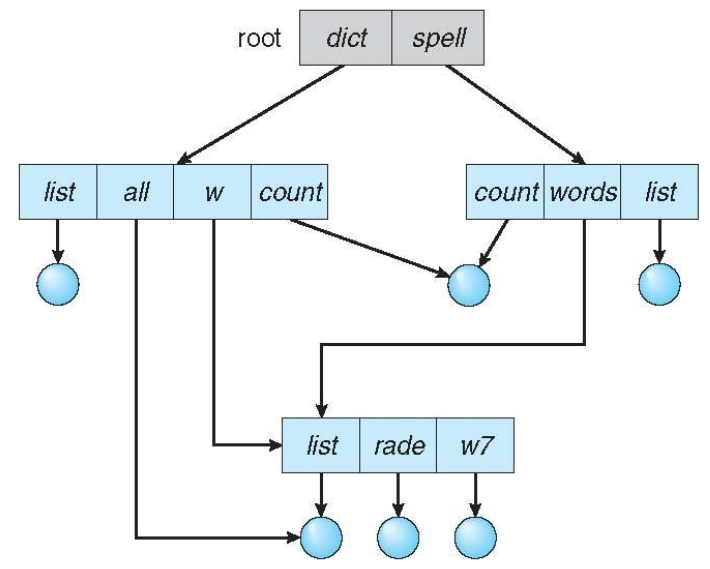
\includegraphics[width=0.5\linewidth]{content/OS_Internals/img/fdbg.png}
\end{figure}

Quando si elimina una directory, si ottiene un puntatore pendente (dangling pointer) che punta a memoria non più allocata; il suo dereferenziamento costituisce un comportamento indefinito.

Soluzioni:

\begin{itemize}
  \item Backpointer, in modo da poter eliminare tutti i puntatori alla cartella eliminata; records di dimensione variabile sono un problema
  \item Backpointer usando un'organizzazione a catena (daisy chain)
  \item Soluzione con contatore di riferimenti (entry-hold-count)
\end{itemize}

Nuovi tipi di voci nelle directory:

\begin{itemize}
  \item[] \textbf{Link} - un altro nome (puntatore) a un file esistente
  \item[] \textbf{Risolvi il link} - segui il puntatore per localizzare il file
\end{itemize}

\newpage
\subsection{Directory a Grafo Generale}

Come garantiamo l'assenza di cicli? Consentiamo solo link a file, non a sottodirectory; \textbf{Garbage collection}; ogni volta che viene aggiunto un nuovo link, si usa un algoritmo di rilevamento dei cicli per verificare se è accettabile.

\begin{figure}[h!]
  \centering
  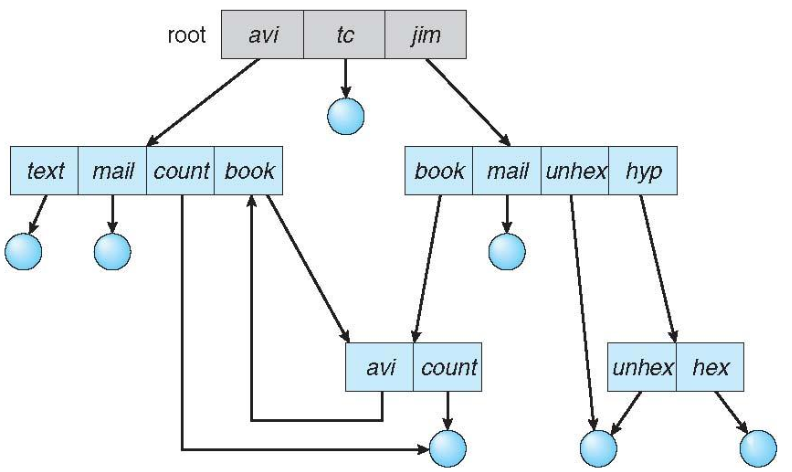
\includegraphics[width=0.55\linewidth]{content/OS_Internals/img/dngf.png}
\end{figure}


\section{File System Mounting}
A file system must be mounted before it can be accessed. A unmounted file system is mounted at a
mount point

\begin{figure}[h!]
  \centering
  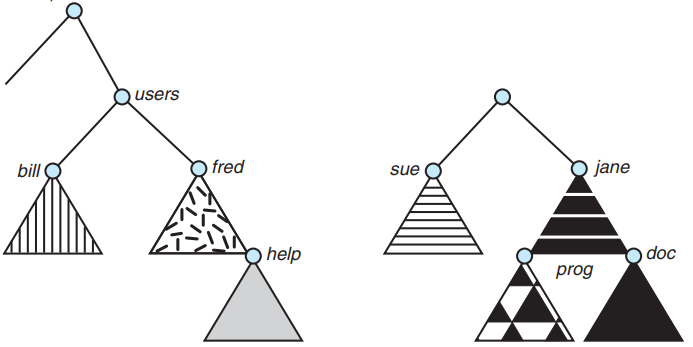
\includegraphics[width=0.5\linewidth]{content/OS_Internals/images/2026-03-22-17-53-56.png}
\end{figure}

\section{File Sharing}

Sharing of files on multi-user systems is desirable.
Sharing may be done through a protection scheme.
On distributed systems, files may be shared across a network.
Network File System (NFS) is a common distributed file-sharing
method.
If multi-user system:

\begin{itemize}
  \item \textbf{User IDs} identify users, allowing permissions and
        protections to be per-user
  \item \textbf{Group IDs} allow users to be in groups, permitting group
        access rights
  \item Owner of a file / directory
  \item Group of a file / directory
\end{itemize}

\subsection{File Sharing - Remote File Systems }

Uses networking to allow file system access between systems

\begin{itemize}
  \item Manually via programs like FTP
  \item Automatically, seamlessly using distributed file systems
  \item Semi automatically via the world wide web
\end{itemize}

Client-server model allows clients to mount remote file systems from
servers:

\begin{itemize}
  \item Server can serve multiple clients
  \item Client and user-on-client identification is insecure or complicated
  \item NFS is standard UNIX client-server file sharing protocol
  \item CIFS is standard Windows protocol
  \item Standard operating system file calls are translated into remote calls
\end{itemize}

Distributed Information Systems (distributed naming services) such
as LDAP, DNS, NIS, Active Directory implement unified access to
information needed for remote computing


\subsection{File Sharing - Failure Modes}

All file systems have failure modes, for example corruption of directory structures or other nonuser data, called metadata.
Remote file systems add new failure modes, due to network
failure, server failure.
Recovery from failure can involve state information about
status of each remote request.

Stateless protocols such as NFS v3 include all information in
each request, allowing easy recovery but less security.


\subsection{File Sharing - Consistency Semantics}

Specify how multiple users are to access a shared file
simultaneously.
Tend to be less complex
due to disk I/O and network latency (for remote file systems). Andrew File
System (AFS) implemented complex remote file sharing semantics. Unix file
system (UFS) implements: ! Writes to an open file visible immediately to other
users of the same open file ! Sharing file pointer to allow multiple users to
read and write concurrently. AFS has session semantics ! Writes only visible to
sessions starting after the file is closed


\section{Protezione}

Il problema:
non si desidera che altri modifichino, leggano o spostino i propri dati/programmi.

\paragraph{}

Il proprietario/creatore del file deve poter controllare: cosa può essere fatto/visto, da chi.
Tipi di accesso: - Lettura - Scrittura - Esecuzione - Aggiunta - Eliminazione - Elenco.

\paragraph{}
Tutti i sistemi operativi forniscono questa opzione di base.

\subsection{Access Lists and Groups}
Mode of access: read, write, execute. Three classes of users on Unix / Linux:

\begin{itemize}
  \item Owner access 7 $\to$ RWX (111)
  \item Group access 6 $\to$ RW- (110)
  \item Public access 1 $\to$ --X (001)
\end{itemize}



\begin{center}
  \begin{minipage}{0.65\linewidth}
    For a particular file (say game) or subdirectory, define an
    appropriate access.
  \end{minipage}%
  \hfill
  \begin{minipage}{0.3\linewidth}
    \centering
    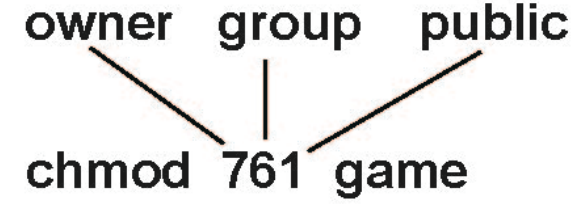
\includegraphics[width=\linewidth]{content/OS_Internals/images/2026-03-22-18-06-47.png}
  \end{minipage}
\end{center}


